%&latex
%
\providecommand{\main}{../..}
\documentclass[../../main.tex]{subfiles}

\begin{document}

%A possible evolution: a class invades the entire lattice (monodominant)
\lesson{35}{28/05/20}
However, we would then need to invert both the Laplace and Fourier transform to get $G(\bm{x},t)$, and finally take the limit for $t \to +\infty$ to see what is the right limiting scenario (monodominance or biodiversity). This can be done, but it is not really necessary to answer our question.

Luckily, just knowing $h(s)$ (\ref{eqn:h-s}) suffices. In fact, from (\ref{eqn:laplacian-term-transformed}) we have:
\begin{align*}
    \frac{h(s)}{L^d} &= -\frac{1}{4} \bigtriangleup_{\bm{x}} \hat{G}(\bm{x},s)  \Big|_{\bm{x}=\bm{0}} \underset{\mathclap{(\ref{eqn:discrete-laplacian})}}{=}  -\frac{1}{4} \sum_{\mu=1}^d \Big[\hat{G}(\bm{\hat{\mu}}, s) + \hat{G}(-\bm{\hat{\mu}},s) - 2\underbrace{\hat{G}(\bm{0},s)}_{1}  \Big] =\\
    &\underset{\mathclap{(\ref{eqn:laplace-transform})}}{=}  \frac{1}{4} \sum_{\mu=1}^d \int_0^\infty \dd{t} e^{-st} \Big[\underbrace{1 - G_t(\bm{\hat{\mu}})}_{C_t\text{ (\ref{eqn:C-t})}} + \underbrace{1 - G_t(-\bm{\hat{\mu}})}_{C_t}   \Big] =\\
    &= \frac{d}{2} \int_0^\infty \dd{t} e^{-st} C_t \equiv \frac{d}{2} \hat{C}(s)  
\end{align*}
So $h(s)$ is proportional to the Laplace transform of the quantity $C_t$ we are interested in. Note that if $s \to 0$, values of $C_t$ with larger $t$. So, to understand the \textit{large} $t$ limit of $C_t$ we can study\footnote{This argument can be made rigorous by using a Tauberian theorem} the behaviour of $\hat{C}(s)$ at small $s$. 

\medskip

So, recall the form of $h(s)$:
\begin{align}\nonumber
    \frac{h(s)}{L^d}  &= \frac{A(s)}{1-A(s)}  2p(1-p) = \frac{d}{2} \hat{C}(s)\\
    A(s) &= \frac{1}{L^d} \sum_{\bm{q}} \frac{2 \lambda(\bm{q}) \textcolor{Red}{+s -s}}{s + 2 \lambda(\bm{q})} = \frac{\cancel{L^d}}{\cancel{L^d}}  - s \frac{1}{L^d} \sum_{\bm{q}} \frac{1}{s+ 2 \lambda(\bm{q})}  \label{eqn:A-of-s}
\end{align}
In particular, note that $A(s) \to 1$ when $s \to 0$, meaning that $h(s)$ is diverging for $s \to 0$. To proceed, we make an expansion:
\begin{align*}
    \frac{d}{2} \hat{C}(s) &= \frac{\overbrace{A(s)}^{\approx 1} }{1 - A(s)} 2p(1-p)  = 2p(1-p) (1 - A(s))^{-1} (1+ O(s)) =\\
    &\underset{\mathclap{(\ref{eqn:A-of-s})}}{=} 2p(1-p) \left[\frac{1}{L^d} \sum_{\bm{q}} \frac{s}{s + 2 \lambda(\bm{q})}  \right]^{-1} (1 + O(s))
\end{align*}
In the continuum limit, the term in the square brackets becomes an integral of the first Brillouin zone $B = [-\pi, \pi]^d$, since $\lambda(\bm{q})$ is periodic in each $q_\mu$:
\begin{align}\label{eqn:bracket-continuum}
    \frac{1}{L^d} \sum_{\bm{q}} \frac{s}{s+ 2\lambda(\bm{q})}   \xrightarrow[L \to +\infty]{}  \int_B \frac{\dd[d]{\bm{q}}}{(2\pi)^d} \frac{s}{s+ 2\lambda(\bm{q})} 
\end{align}
Recall that $\lambda(\bm{0}) = \bm{0}$, and so it will be \textit{small} when $\bm{q} \to \bm{0}$. So for \textit{small} $s$, the denominator is small when $\bm{q} \to \bm{0}$, meaning that the integral is dominated by small values of $\bm{q}$.

Thus we expand $\lambda(\bm{q})$ around $\bm{q} = 0$:
\begin{align}\label{eqn:lambda-expansion}
    2 \lambda(\bm{q}) &= \sum_{\mu=1}^d (1- \cos q_\mu) \underset{\mathclap{q_\mu \approx 0}}{=}\> \frac{1}{2} \sum_{\mu} (q_\mu^2 + O(q_\mu^4)) = \frac{\norm{\bm{q}}^2}{2} + O(q_\mu^4)
\end{align} %TODO Is this necessary?
and consider (\ref{eqn:bracket-continuum}) when $s \to 0$:
\begin{align*}
    \int_B \frac{\dd[d]{\bm{q}}}{(2\pi)^d} \frac{1}{2 \lambda(\bm{q})} \equiv J_d
\end{align*}
We use the fact that $1 - \cos x \geq x^2/4$ for $|x| < l$, where $l$ is the solution of $1-\cos l - l^2 = 0$. Then we split the integral domain $B$ in the region $B' = [-l,l]^d$ and the rest $B-B'$:
\begin{align*}
    J_d \equiv \int_B \frac{\dd[d]{\bm{q}}}{(2\pi)^d} \frac{1}{2 \lambda(\bm{q})} &= \int_{B'} \frac{\dd[d]{\bm{q}}}{(2 \pi)^d} \frac{1}{2 \lambda(\bm{q})} + \int_{B - B'} \frac{\dd[d]{\bm{q}}}{(2\pi)^d} \frac{1}{2 \lambda(\bm{q})} \\
    &\leq 4 \underbrace{\int_{B'} \frac{\dd[d]{\bm{q}}}{(2\pi)^d} \frac{1}{\norm{\bm{q}}^2}}_{\displaystyle < \infty \text{if $d > 2$}}\quad  +  \quad\underbrace{\int_{B - B'} \frac{\dd[d]{\bm{q}}}{(2\pi)^d}   \frac{1}{2 \lambda(\bm{q})} }_{\mathclap{\displaystyle  < \infty \> \forall d \text{ since } \inf_{\mathclap{q \in B - B'}} \lambda(\bm{q}) > 0}}
\end{align*}
To prove that the first term is finite for $d > 2$ we can use polar coordinates in $d$ dimensions:
\begin{align*}
    \int_{B'} \dd[d]{\bm{q}} \frac{1}{\norm{\bm{q}}^2} \leq \int_{\norm{\bm{q}} < 2l}  \dd[d]{\bm{q}} \frac{1}{\norm{\bm{q}}^2} = \int \underbrace{\dd{\Omega_d} }_{\parbox[c]{4em}{\footnotesize$d$-dim spherical surface}} \int_0^{2l} q^{d-3} \dd{q} {<}  \infty \text{\ \ if $d-2>0$}
\end{align*}
Thus, if $d > 2$, $J_d < \infty$, meaning that when $d > 2$ and $s \approx 0$:
\begin{align*}
    \frac{1}{L_d} \sum_{\bm{q}} \frac{s}{s + 2 \lambda(\bm{q})}  \xrightarrow[L \to +\infty]{} \int_B \frac{\dd[d]{\bm{q}}}{(2\pi)^d} \frac{s}{s + 2 \lambda(\bm{q})} = s J_d (1 + o(s))  
\end{align*}
And taking the reciprocal:
\begin{align}\label{eqn:C-transform}
    \hat{C}(s) = \int_0^\infty e^{-st} C_t \dd{t} = \frac{4p(1-p)}{d J_d} \frac{1}{s} (1 + o(s)) \qquad d > 2
\end{align}

Suppose that:
\begin{align*}
    \lim_{t \to +\infty} C_t = C_\infty
\end{align*}
Since $0 < C_t \leq 1$ (\ref{eqn:C-t}), we have:
\begin{align}\label{eqn:C-limit}
    \hat{C}(s) = \int_0^\infty e^{-ts} C_t \dd{t} \underset{z = ts}{=} \frac{1}{s} \int_0^\infty e^{-z} C_{z/s} \dd{z}   \underset{s \approx 0}{\approx} \frac{1}{s} C_\infty
\end{align}
because:
\begin{align*}
    \int_0^\infty e^{-z} C_{z/s} \dd{z} \xrightarrow[s \to 0]{} \int_0^\infty e^{-z} C_{\infty} \dd{z} = C_\infty
\end{align*}
due to the Lebesgue dominated convergence theorem.

\medskip

Finally, substituting (\ref{eqn:C-limit}) in (\ref{eqn:C-transform}) for $s \approx 0$ leads to:
\begin{align*}
    \frac{C_\infty}{\cancel{s}} =  \frac{4p(1-p)}{d J_d} \frac{1}{\cancel{s}} \Rightarrow C_{\infty} = \frac{4 p(1-p)}{d \cdot J_d} > 0 \qquad d > 2
\end{align*}
Recalling the definition of $C_t$ (\ref{eqn:C-t}), this proves that, for $d > 2$, the system tends to a state with \textit{many species} \q{well mixed} together (biodiversity), as in fig. \ref{fig:dispersion}.

\medskip

If $d < 2$, the integral in (\ref{eqn:bracket-continuum}) is still dominated by the behaviour of $\lambda(\bm{q})$ at small $\bm{q}$, but in a rather different way. By using the expansion (\ref{eqn:lambda-expansion}) we get:
\begin{align*}
    \int_B \frac{\dd[d]{\bm{q}}}{(2\pi)^d} \frac{s}{s+2\lambda(\bm{q})}  &\underset{\mathclap{(\ref{eqn:lambda-expansion})}}{\approx} s \int_B \frac{\dd[d]{\bm{q}}}{(2\pi)^d} \frac{1}{s+ \norm{\bm{q}}^2/s}   \underset{\bm{q} = \bm{x}\sqrt{s}}{=} s^{d/2} \int_{\frac{B}{\sqrt{s}}} \frac{1}{1+\norm{\bm{x}}^2/2} \frac{\dd[d]{\bm{x}}}{(2\pi)^d} =\\
    &\underset{\mathclap{s \approx 0}}{=}  s^{d/2} \underbrace{\int_{\mathbb{R}^d} \frac{\dd[d]{\bm{x}}}{(2\pi)^d} \frac{1}{1+\frac{\norm{\bm{x}}^2}{2} }}_{K_d}   (1 + o(s))
\end{align*}
where the integral $K_d$ converges in $d < 2$. Then for $\hat{C}(s)$ is proportional to the reciprocal:
\begin{align*}
    \hat{C}(s) = \frac{4p(1-p)}{K_d d} s^{-d/2} (1+o(s)) 
\end{align*}
which is the Laplace transform of:
\begin{align*}
    C_t = \frac{4p(1-p)}{d K_d} \Gamma\left(\frac{d}{2} \right) t^{\frac{d}{2}-1}  \xrightarrow[t \to +\infty]{}  0 \qquad d < 2
\end{align*}
In fact, it can be shown that:
\begin{align*}
    \int_0^\infty e^{-st} t^{\frac{d}{2}-1} \dd{t} = s^{-\frac{d}{2} } \Gamma\left(\frac{d}{2} \right)
\end{align*}
Since $C_t  \xrightarrow[t \to \infty]{} 0$ for $d<2$, the final scenario will be the one where a single species occupies all the lattice (monodominance).

\medskip

Finally, for the $d=2$ case we proceed similarly:
\begin{align*}
    \int_{[-\pi, \pi]^2} \dd[2]{\bm{q}} \frac{s}{s+2\lambda(\bm{q})}  &\underset{\mathclap{s\approx 0}}{\approx} s \int_{[-\pi, \pi]^2} \dd[2]{\bm{q}} \frac{1}{s+ \norm{\bm{q}}^2/2}  \underset{\bm{q}=\bm{x}\sqrt{s}}{=} s \int_{\norm{\bm{x}} < \pi/\sqrt{s}} \frac{\dd[2]{\bm{x}}}{1 + \norm{\bm{x}}/2} =\\
    &=  2 \pi s \int_0^{\frac{\pi}{\sqrt{s}}} \frac{x \dd{x}}{1 + x^2/2} = 2 \pi s \ln \left(1+\frac{\pi^2}{2 s} \right) =\\
    &\approx 2 \pi s |\ln s| \left(1+ O\left(\frac{1}{|\ln s|} \right)\right) \propto \frac{1}{\hat{C}(s)} 
\end{align*}
And its Laplace anti-transform is proportional to:
\begin{align*}
    C_t \propto \frac{1}{\ln t} 
\end{align*}
In fact:
\begin{align*}
    \int_0^\infty e^{-st} \frac{1}{\ln t}  \dd{t} &\underset{st = z}{=}  \frac{1}{s} \int_0^\infty \frac{e^{-z}}{\ln z - \ln s} \dd{z} =\\
    &\underset{s \approx 0}{=}   \frac{1}{s |\ln s|} \int_0^\infty \frac{e^{-z}}{1 + \frac{\ln z}{|\ln s|} } \dd{z} \approx \frac{1}{s |\ln s|} 
\end{align*}
since by the Lebesgue's dominated convergence theorem:
\begin{align*}
    \lim_{s \to 0} \int_0^\infty \frac{e^{-z}}{1 + \frac{\ln z}{|\ln s|} } \dd{z} = \int_0^\infty e^{-z} \dd{z} = 1
\end{align*}
At the end, $C_t \propto 1/\ln t  \xrightarrow[t \to +\infty]{}  0$, and so also in the $d=2$ case the model predicts a scenario of \textit{monodominance}. However, $C_t$ goes to $0$ \textit{very slowly}, so if the system's timescale is long enough, we can still observe (temporarily) a scenario of \textit{biodiversity}.

\medskip

In summary:
\begin{align}\label{eqn:scaling-2-point-corr}
    C_t \underset{t \gg 1/w}{\sim} \begin{cases}
        C_\infty & d > 2 \qquad \text{(Biodiversity)}\\
        \frac{1}{\ln t} & d = 2 \qquad \text{(Monodominance)} \\
        t^{\frac{d}{2} - 1} & d < 2 \qquad \text{(Monodominance)}
    \end{cases}
\end{align}

\begin{exo}[Mean Field for Voter Model]
    Consider a voter model where each node can interact with \textbf{every} other.
    
    \begin{enumerate}
        \item Determine the transition rate $W(n+1|n)$ ($n \to n+1$) and $W(n-1|n)$ ($n \to n-1$).
        \item Write the Master Equation $\mathbb{P}(n;t)$ for the probability to have a species with population $n$ at time $t$.
        \item Calculate $\langle n \rangle_t$ and $\langle n^2 \rangle_t$.
    \end{enumerate}
\end{exo}

\subsection{Final Remarks}
The voter model we just examined is \textit{non-parametric} - the only parameter we inserted is $w$, which is just the reciprocal of a timescale, and so does not have any qualitative impact on the dynamics. Nonetheless, we see some scaling behaviour, for example for the $2$-point correlation function (\ref{eqn:scaling-2-point-corr}), which is typical of systems near \textbf{criticality}. 

So, in a sense, the voter model \q{needs no tuning} to be near a critical point - which is exactly what happens in natural systems.

\section{Contact Process}
The last model we consider is the \textbf{Contact Process}, originally proposed by T. E. Harris as a toy model for describing an epidemic. It is a sort of \q{Ising model} for describing \textbf{dynamical transitions} in non-equilibrium systems. 

\medskip

As usual, we consider nodes $\bm{x} \in \mathbb{Z}^d$ in a $d$-dimensional cubic lattice. Each node can be either 
\textcolor{Blue}{healthy}  ($\sigma_x = 0$) or \textcolor{Red}{infected} ($\sigma_x = 1$):
\begin{align*}
    \sigma_x = \begin{cases}
        \textcolor{Red}{1} & \text{if node $x$ is \textcolor{Red}{infected}}\\
        \textcolor{Blue}{0} & \text{if node $x$ is \textcolor{Blue}{healthy}}
    \end{cases}
\end{align*}
The dynamics is given by the following rules:
\begin{itemize}
    \item \textbf{Infection}. Infected nodes \textit{propagate the infection} to their nearest neighbours at a rate $\lambda/2d$. 
    \item \textbf{Recovery}. Infected nodes recover at a unit rate, and are immediately susceptible to a re-infection. 
\end{itemize}

\begin{figure}[H]
    \centering
    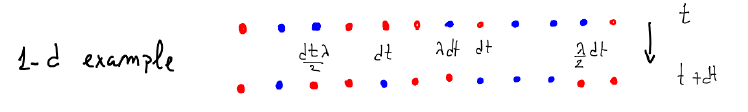
\includegraphics[width=0.9\textwidth]{\main/Images/contact-process.png}
    \caption{Example of evolution for a $d=1$ contact process during a single timestep.}
    \label{fig:contact-process}
\end{figure}
The state where every node is \textit{healthy} is an \textbf{absorbing state}, since nobody will ever get infected again. On the other hand, the state where everyone is \textit{infected} is not absorbing, as infected individuals can recover.

\medskip

So, in the limit $t \to +\infty$, the system can be in one of two different scenarios, depending on the choice of $\lambda$:
\begin{enumerate}
    \item \textbf{Non-active phase}. The absorbing state is reached, meaning that the epidemic \q{becomes extinct}.
    \item \textbf{Active phase}. The epidemic persists with a constant density of infected nodes.
\end{enumerate}

Note that the second scenario can happen only on a \textbf{infinitely large} system (thermodynamic limit), since for any finite number of nodes there is a always a non-zero probability for all nodes to recover at the same time.

In the limit $t \to +\infty$, this event will happen with certainty, and so the only possible scenario is the first one. What it's interesting, is then to compute the \textit{time} needed to reach the absorbing state - which is expected to \textit{scale} with the number of nodes. The exact form of this scaling depends on $\lambda$. It can be shown that, for a $\lambda > \lambda_c$, the extinction time scales \textit{exponentially} in the number $N$ of nodes, but for $\lambda \approx \lambda_c$ it scales according to a \textit{power law}.

\subsection{Infinite range model}
Let's consider a \textit{mean field} version of the model, where the population is \q{well mixed}, meaning that each individual is nearest neighbour with \textbf{every} other node. 

\medskip

Then, denoting with $N$ the total number of nodes and with $n$ the number of infected ones, the Master Equation is that of a birth-death process:
\begin{align}\label{eqn:contact-ME}
    \dot{\mathbb{P}}(n;t) = b(n-1) \mathbb{P}(n-1;t) + d(n+1;t) - (b(n) + d(n)) \mathbb{P}(n;t) \qquad n \geq 0
\end{align}
with $d(N+1) = b(-1) \equiv 0$ and \q{absorbing boundaries} $\mathbb{P}(-1;t) = \mathbb{P}(N+1;t) = 0$

\medskip

$b(n)$ is the rate at which new people get infected (transition $n \to n+1$).
Each pair of susceptible-infected nodes contributes to $b(n)$ with a rate $\lambda/(N-1)$, since $N-1$ is the number of nearest neighbours of each node. As there are $n \cdot (N-n)$ possible pairs (each of the $n$ infected can spread the illness to each of the $N-n$ healthy ones), we get:
\begin{align}\label{eqn:bofn}
    b(n) \equiv W(n+1|n) = \frac{\lambda}{n-1} n (N-n) 
\end{align}
On the other hand, $d(n)$ is the rate at which infected recover (transition $n \to n-1$). Each infected has a unit rate of recovery, and there are $n$ infected, meaning that:
\begin{align}\label{eqn:dofn}
    d(n) \equiv W(n-1|n) = n
\end{align}
The evolution of the average number of infected nodes $\langle n \rangle_t$ at time $t$ is given by:
\begin{align*}
    \dv{t} \langle n \rangle_t &= \sum_{n=0}^N \dot{\mathbb{P}}(n;t) n =\\
    &\underset{\mathclap{(\ref{eqn:contact-ME})}}{=} \> \sum_{n=0}^N n [b(n-1) \mathbb{P}(n-1;t) + d(n+1)\mathbb{P}(n+1;t) - (d(n) + b(n)) \mathbb{P}(n;t)] =\\
\intertext{Then we shift indices in the first and second term, so that $b(n-1) \to b(n)$ and $d(n+1) \to d(n)$:}
    &= \sum_{n=\textcolor{Red}{-1}}^{N\textcolor{Red}{-1}} (n\textcolor{Red}{+1}) b(n) \mathbb{P}(n;t) + \sum_{n=\textcolor{Red}{1}}^{N\textcolor{Red}{+1}} (n\textcolor{Red}{-1}) d(n) \mathbb{P}(n;t) - \sum_{n=0}^N n(d(n) + b(n)) \mathbb{P}(n;t) =\\
\intertext{Since $b(N) = b(-1) = d(0) = d(N+1) = 0$ we can make all sums go from $0$ to $N$, and collect everything together:}
    &= \sum_{n=\textcolor{Red}{0}}^{\textcolor{Red}{N}} \Big[ (\cancel{n}+1) b(n) \mathbb{P}(n;t) + (\bcancel{n}-1) d(n) \mathbb{P}(n;t) - n(\bcancel{d(n)} + \cancel{b(n)}) \mathbb{P}(n;t) \Big] =\\
    &= \sum_{n=0}^N [b(n) - d(n)] \mathbb{P}(n;t) = \langle b(n) - d(n) \rangle_t \underset{\mathclap{\substack{(\ref{eqn:bofn})\\(\ref{eqn:dofn})}}}{=} \frac{\lambda}{N-1} \langle n(N-n) \rangle _t - \langle n \rangle_t
\end{align*}
Thus we arrive to:
\begin{align}\label{eqn:contact-evo1}
    \dv{t} \langle n \rangle_t = \frac{\lambda}{N-1} \langle n(N-n) \rangle_t - \langle n \rangle_t
\end{align}
For large $N$, $\lambda/(N-1) \approx \lambda/N$. Then we divide both sides by $N$, and define the \textbf{density} of infected $\rho(t) \equiv \langle n/N \rangle_t$:
\begin{align}\label{eqn:contact-evo2}
    \dot{\rho} = \lambda \langle \frac{n}{N} \left(1- \frac{n}{N} \right)  \rangle_t - \rho = (\lambda - 1)\rho - \lambda \langle \left(\frac{n}{N} \right)^2 \rangle_t
\end{align}
To solve (\ref{eqn:contact-evo2}) we need to determine how $\langle (n/N)^2 \rangle_t$ evolves, but this would require knowing $\langle (n/N)^3 \rangle_t$ and so on, leading to an entangled hierarchy of differential equations.

\medskip

To proceed, we use a \textbf{mean field approximation}, factorizing the average:
\begin{align}\label{eqn:contact-mf}
    \langle \left(\frac{n}{N} \right)^2 \rangle_t \approx \langle \frac{n}{N}  \rangle^2_t = \rho^2(t)
\end{align} 
However, note that this introduces a \textit{systematic error} in our model, since:
\begin{align}\label{eqn:var-term}
    \langle \left(\frac{n}{N} \right)^2 \rangle_t - \langle \frac{n}{N}  \rangle^2_t = \Big(\operatorname{Var} \frac{n}{N} \Big)_t \geq 0
\end{align} 

Substituting (\ref{eqn:contact-mf}) in (\ref{eqn:contact-evo2}) leads to:
\begin{align}\label{eqn:contact-evo3}
    \dot{\rho} = (\lambda - 1) \rho - \lambda \rho^2
\end{align}

Let's start by analyzing the stationary state. We have two cases:
\begin{itemize}
    \item $\lambda < 1 \equiv \lambda_c$. In this case all the right hand side of (\ref{eqn:contact-evo3}) is negative, meaning that $\rho$ is always decreasing. Since $\rho \geq 0$, the final (stationary) state will be $\rho^* = 0$.
    
    \medskip

    Analytically, if we set $\dot{\rho} \overset{!}{=} 0$:
    \begin{align*}
        \rho^* \colon (\lambda - 1) \rho^* - \lambda (\rho^*)^2 \overset{!}{=}  0 \Leftrightarrow \rho^* = 0 \> \lor \> \rho^* = \frac{\lambda-1}{\lambda} < 0 
    \end{align*}
    and the negative solution is unphysical.

    \medskip

    Due to the form of (\ref{eqn:contact-evo3}), the absorbing state $\rho=0$ will be reached \textit{exponentially fast} (fig. \ref{fig:rho-1}).
    \item $\lambda > 1 \equiv \lambda_c$. In this case we still have $\rho^* = 0$, but also $\rho^* = (\lambda -1)/\lambda \equiv \bar{\rho} > 0$. Studying the sign of (\ref{eqn:contact-evo3}), we have that for any initial $\rho_0 \in (0,1]$, the final stationary state will be $\bar{\rho}$, and only for $\rho_0 = 0$ we will have $\rho^* = 0$ instead (fig. \ref{fig:rho-2}).

    \medskip

    This is true only for an infinite system, where the fluctuations (\ref{eqn:var-term}) are null. For any finite system, $\rho$ will initially tend to $\bar{\rho}$, but given a sufficient time, some stochastic fluctuation will cause it to reach $0$, where it will remain forever.
\end{itemize}

\begin{figure}[H]
    \centering
    \begin{subfigure}[t]{0.45\textwidth}
        \centering
        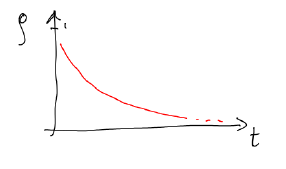
\includegraphics[width=\textwidth]{\main/Images/rho1.png}
        \caption{$\lambda < 1 \equiv \lambda_c$}
        \label{fig:rho-1}
    \end{subfigure}
    \hfill
    \begin{subfigure}[t]{0.45\textwidth}
        \centering
        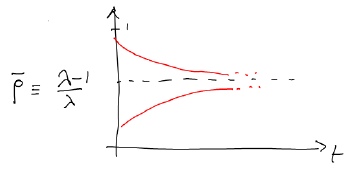
\includegraphics[width=\textwidth]{\main/Images/rho2.png}
        \caption{$ \lambda > 1 \equiv \lambda_c$}
        \label{fig:rho-2}
    \end{subfigure}
       \caption{Evolution of the infected density $\rho$ below and above the critical rate $\lambda_c$. For $\lambda < \lambda_c = 1$, the epidemic becomes extinct, but for $\lambda > \lambda_c$ it \q{survives} forever with a constant density of infected $\bar{\rho}$ (assuming an infinite system).}
       \label{fig:rho1-2}
\end{figure}

We can then explicitly solve (\ref{eqn:contact-evo3}) by separation of variables, with the initial condition $\rho(0) \equiv \rho_0$:
\begin{align*}
    \rho(t) = \frac{\Delta}{\lambda + \frac{\Delta - \lambda \rho_0}{\rho_0} e^{- \Delta\cdot  t}} \qquad \Delta = \lambda - 1 \equiv \lambda - \lambda_c \neq 0
\end{align*}
For times well above the characteristic timescale ($t \gg |\Delta|^{-1} \equiv \tau_c$), we see that the density approaches the stationary solution \textit{exponentially fast}:
\begin{align*}
    \rho(t) \> &\underset{\mathclap{t \gg \tau_c}}{\sim}  \> e^{-|\Delta| t} \qquad \Delta < 0\\
    \rho(t) - \bar{\rho} \> &\underset{\mathclap{t \gg \tau_c}}{\sim}  \> e^{-|\Delta| t} \qquad \Delta > 0
\end{align*} 

%TODO Prove these two relations

The system's phase diagram is shown in fig. \ref{fig:diagram-contact}. 

\begin{figure}[H]
    \centering
    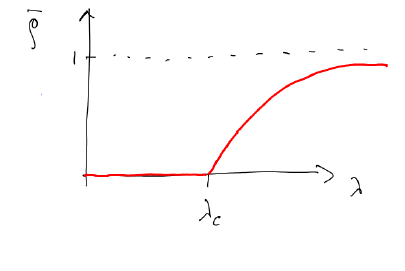
\includegraphics[width=0.7\textwidth]{\main/Images/diagram-contact.png}
    \caption{Phase diagram for the \textit{mean field} contact process. The stationary density $\bar{\rho}$ is $0$ for $\lambda < \lambda_c$, and starts to approach $1$ when $\lambda > \lambda_c$.}
    \label{fig:diagram-contact}
\end{figure}

In particular we observe, in the mean field approximation:
\begin{align*}
    \bar{\rho} \propto \Delta^{\textcolor{Red}{\beta}} \qquad \beta = 1; \quad \Delta > 0 
\end{align*}
and the system's timescale is $\tau = |\Delta|^{-\textcolor{Red}{1}}$.

\medskip

The contact system behaves \textit{similarly} to the Ising Model, with the stationary density $\bar{\rho}$ assuming the role of the magnetization $m$. Some key differences are:
\begin{itemize}
    \item In the Mean Field IM, the scaling exponent is $\beta = 1/2$ and not $1$.
    \item This is a \textbf{dynamical} transition, not an equilibrium one. In fact, the contact process is \textit{never} at equilibrium (there are no Boltzmann weights, nor detailed balance). Also, when $\lambda < \lambda_c$, the stationary state is $\bar{\rho} = 0$ - without any kind of fluctuation. In this case, the system experiences \textit{no dynamics at all} - which is quite different from what happens in the high temperature phase of the IM.   
\end{itemize}
 
All that's left is the $\Delta = 0$ case, when $\lambda = \lambda_c = 1$. Equation (\ref{eqn:contact-evo3}) becomes:
\begin{align*}
    \dot{\rho} = - \rho^2
\end{align*}
which can be immediately integrated, leading to:
\begin{align*}
    \rho(t) = \frac{\rho_0}{1 + t \rho_0} \underset{t \gg \tau_c}{\sim}  t^{\textcolor{Red}{-1}} 
\end{align*}
which is a power-law behaviour. In particular, note that $\rho(t)$ approaches $\bar{\rho}$ \textit{much more slowly} than in all other cases, where the decay is exponential. This is again the phenomenon of \textbf{critical slowing down}. 












\end{document}
 
